% !TeX program = pdflatex
\documentclass{IEEEtran}
\usepackage{latexsym}
\usepackage{graphicx}
\usepackage{amsfonts,amssymb,amsmath}
\usepackage{hyperref}
\usepackage{cleveref}
\def\BibTeX{{\rm B\kern-.05em{\sc i\kern-.025em b}\kern-.08em T\kern-.1667em\lower.7ex\hbox{E}\kern-.125emX}}
\markboth{$>$ REPLACE THIS LINE WITH YOUR PAPER IDENTIFICATION NUMBER $<$}
{$>$ REPLACE THIS LINE WITH YOUR PAPER IDENTIFICATION NUMBER $<$}
\begin{document}

\title{Stable Structures for Nonlinear Biquad Filters}

\author{Jatin Chowdhury
\thanks{Manuscript received November 21, 2019.}
\thanks{The author is with 
the Center for Computer Research in Music and Acoustics (CCRMA),
Stanford University, Stanford, CA 
94305 USA, (e-mail: jatin@ccrma.stanford.edu).}}


\IEEEtitleabstractindextext{\begin{abstract}
    Biquad filters are a common tool for filter design. In this
    writing, we develop two structures for creating biquad filters
    with nonlinear elements. We provide conditions for the guaranteed
    stability of the nonlinear filters, and derive expressions for
    instantaneous pole analysis. Finally, we examine example filters
    built with these nonlinear structures, and show how the first
    nonlinear structure can be used in the context of analog modelling.
\end{abstract}

\begin{IEEEkeywords}
    Audio systems, digital filters, nonlinear filters, stability analysis.
\end{IEEEkeywords}}

\maketitle
\IEEEdisplaynontitleabstractindextext

\section{Introduction}
A ``biquad'' filter refers to a general 2nd order IIR filter.
In digital signal processing, biquad filters are often useful
since any higher-order filter can be implemented using a cascade
of biquad filters. While digital biquad filters are typically implemented
as linear processors, for audio applications it can be useful to
implement nonlinear filters. For example, in \cite{SKF} the authors
use a passive model of operational amplifiers to model the nonlinear
behaviour of a Sallen-Key lowpass filter. Meanwhile, in \cite{Vadim},
the author proposes several methods for using nonlinear elements
to enhance linear models of analog ladder filters. More relevant to
our current topic is \cite{Rossum1992MakingDF}, in which the author
suggests a method for altering a general digital feedback filter
by saturating the feedback path, with the goal of achieving a more
analog-like response. In this writing, we strive
to develop more general nonlinear filter structures. While these structures
may be used for analog modelling, they do not necessarily depend on analog
modelling principles to be understood and implemented.

\section{Structural Elements}
\subsection{Linear Filter}
%
We begin with the equation for a biquad filter:
%
\begin{equation}
\begin{split}
    y[n] = b_0 u[n] + b_1 u[n-1] + b_2 u[n-2] \\ - a_1 y[n-1] - a_2 y[n-2]
\end{split}
    \label{eq:bq}
\end{equation}
%
Where $y$ is the output signal, $u$ is the input signal, and $a_n$ and $b_n$
are the feed-back and feed-forward filter coefficients, respectively.
There are several convenient ``direct forms'' for implementing biquad filters.
In this writing we will focus on the ``Transposed Direct Form II'' (TDF-II),
which is popular for its numerical properties \cite{JOSFilters}.
%
\begin{figure}[ht]
    \center
    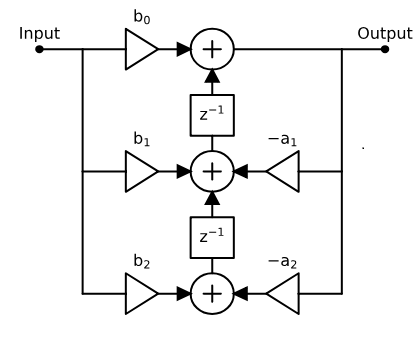
\includegraphics[width=2.3in]{../Pics/TDF-II-White.png}
    \caption{\label{TDF-II}{\it Transposed Direct Form II}}
\end{figure}
%
Note that the poles of the filter can be described using the quadratic
equation.
\begin{equation}
    p = \frac{-a_1 \pm \sqrt{a_1^2- 4a_2}}{2}
    \label{eq:poles_lin}
\end{equation}
%
Specifically, the pole magnitude is described by (ignoring the
trivial case where the poles are strictly real):
\begin{equation}
    |p|^2 = a_2
    \label{eq:poles_lin_mag}
\end{equation}
%
And the angular frequencies of the poles are equal to:
\begin{equation}
    \angle p = \arctan \left( \pm \frac{\sqrt{4a_2 - a_1^2}}{a_1} \right)
    \label{eq:poles_lin_angle}
\end{equation}
%
It is well known that a digital filter will be stable provided that
the magnitudes of the poles are strictly less 1 \cite{JOSFilters}.
\newline
%
\subsubsection{State Space Formulation}

Another reason TDF-II is useful for implementing biquad filters
is that its behavior can easily be written in state space form.
First we define two state variables, at the locations of the delay
elements:
%
\begin{equation}
    \begin{split}
        x_1[n] &= b_1 u[n] - a_1 y[n] + x_2[n-1] \\
        x_2[n] &= b_2 u[n] - a_2 y[n]
    \end{split}
    \label{eq:bq_lin_states}
\end{equation}
%
Then the output of the filter can be written in terms of the states
as
%
\begin{equation}
    y[n] = b_0 u[n] + x_1[n-1]
    \label{eq:state_output_lin}
\end{equation}
%
Finally, we can write the filter equation in a state space form:
%
\begin{equation}
    \begin{bmatrix} x_1[n+1] \\ x_2[n+1] \\ y[n+1] \end{bmatrix} =
    \begin{bmatrix} 0& 1& -a_1\\ 0& 0& -a_2\\ 1& 0& 0 \end{bmatrix}
    \begin{bmatrix} x_1[n] \\ x_2[n] \\ y[n] \end{bmatrix}
    + \begin{bmatrix} b_1\\ b_2\\ b_0 \end{bmatrix} u[n]
    \label{eq:bq_lin_state_spaces}
\end{equation}

\subsection{Nonlinear Elements}
%
We now propose adding nonlinear elements to the above filter structure.
We will refer to these nonlinear elements as ``base nonlinearities''.
To keep the discussion as broad as possible, we consider any one-to-one
nonlinear function $f_{NL}(x)$.
\newline\newline
%
\begin{figure}[!ht]
    \center
    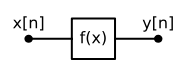
\includegraphics[width=1.0in]{../Pics/NL_sys_trim_white.png}
    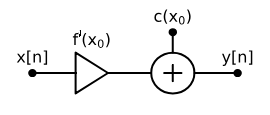
\includegraphics[width=1.4in]{../Pics/NL_sys_lin_white.png}
    \caption{\label{linize}{\it A general digital nonlinear system (left),
                                and a general linearization of that system (right).}}
\end{figure}
%
In analog modelling literature, it is typical to analyze a nonlinear
system by "linearizing" the system about a certain operating
point. This process is typically done by constructing a Thevenin or
Norton equivalent circuit that represents the nonlinear function at
that operating point, where the resistance of the equivalent circuit
is determined by the slope of the nonlinearity at the operating point,
and the source of the equivalent circuit is determined by the DC
offset of the linearized system at the operating point
\cite{BernersDAFX}.
\newline\newline
In our purely digital formulation, we can linearize a nonlinear function
as a gain element plus a constant source (see \cref{linize}).
%
For operating point $x_0$:
%
\begin{equation}
    \bar{f}_{NL}(x) = f'_{NL}(x_0)x + c(x_0)
    \label{eq:linearized}
\end{equation}
%
where the offset $c(x_0)$ is described by
%
\begin{equation}
    c(x_0) = f_{NL}(x_0) - f'_{NL}(x_0)x_0
    \label{eq:lin_off}
\end{equation}
%
In \cref{tanh_lin}, we show an example of linearizing the nonlinear
function $f_{NL}(x) = \tanh(x)$ at $x_0=1$.
%
\begin{figure}[h]
    \center
    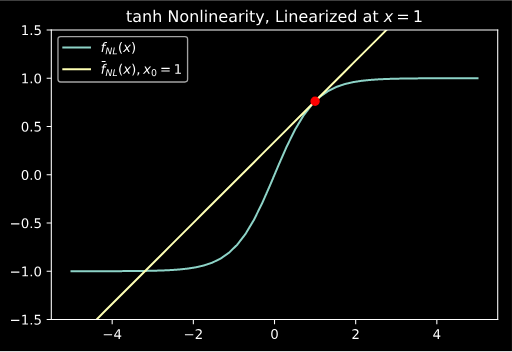
\includegraphics[width=3in]{../Pics/tanh_linized.png}
    \caption{\label{tanh_lin}{\it $\tanh$ nonlinearity, linearized at $x=1$.}}
\end{figure}
%
\subsubsection{Stability Constraints}

In order to guarantee that the filters we construct in the next section
will be stable, we propose the following constraint on the base
nonlinearities used to construct nonlinear filters:
%
\begin{equation}
    \left| f'_{NL}(x) \right| \leq 1
    \label{eq:NL_constraint}
\end{equation}
%
In other words, the nonlinearities must never have
a slope greater than 1. Many typical musical nonlinearities satisfy
this constraint, including many saturating, dropout, rectifying,
and wavefolding nonlinearities. Note that this property is not satisfied by
nonlinear functions that have discontinuous derivatives, such as
$f_{NL}(x) = |x|$. For functions of this type, we recommend using a
smoothing scheme, such as BLAMP \cite{BLAMP}, to achieve a continuous
first derivative.
\newline\newline
Of particular interest to us will be saturating
nonlinearities, including hard-clippers, soft-clippers, and sigmoid-like
functions (see \cref{Sats}).
Saturating nonlinearities satisfy the property that
%
\begin{equation}
    |x| \rightarrow \infty, \ f'_{sat}(x) \rightarrow 0
    \label{eq:Sat_constraint}
\end{equation}
%
\begin{figure}[h]
    \center
    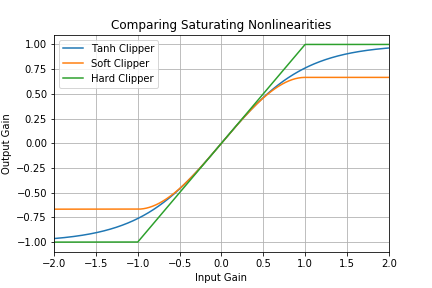
\includegraphics[width=3in]{../Pics/Sat-NLs.png}
    \caption{\label{Sats}{\it Saturating Nonlinearities}}
\end{figure}
%
\subsection{Lyapunov Stability}
%
As mentioned earlier, we can easily tell if a linear system is stable
by analyzing the pole locations. For nonlinear systems, we need a
more robust tool for analyzing stability; in this writing, we use
Lyapunov stability \cite{Lyapunov}, as has previously been applied
to nonlinear digital waveguide networks \cite{JOS-Waveguide}, and
fixed-point direct form filters \cite{LyapunovFixedPointFilters}. To
demonstrate that a system is Lyapunov stable, we must form the discrete
time state space equation of the system:
%
\begin{equation}
    \mathbf{x}[n+1] = \mathbf{f}(\mathbf{x}[n])
    \label{eq:lyapunov_general}
\end{equation}
%
If every element of the Jacobian matrix of $\mathbf{f}$ is less than 1,
at some operating point of the system, then the system is considered
Lyapunov stable about that point.

\section{Nonlinear Filter Structure 1: Nonlinear Biquad}
%
\begin{figure}[ht]
    \center
    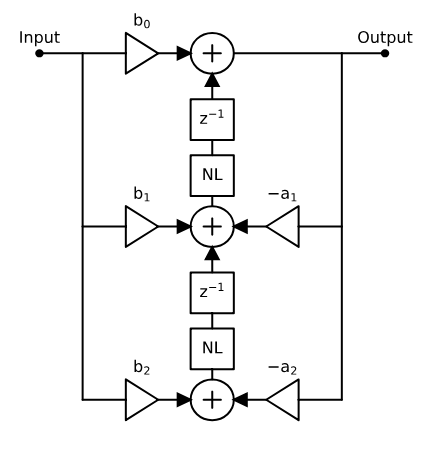
\includegraphics[width=2.3in]{../Pics/NL-TDF-II-White.png}
    \caption{\label{NL-TDF-II}{\it Nonlinear Transposed Direct Form II.
                                The ``NL'' blocks refer to a generalized
                                nonlinear element.}}
\end{figure}
%
We now propose adding nonlinear elements to the TDF-II strcuture in the
following fashion (see \cref{NL-TDF-II}). We will refer to this structure
as the ``Nonlinear Biquad''.
%
The equation for the nonlinear biquad filter then becomes:
%
\begin{equation}
\begin{split}
    y[n] = b_0 u[n]
         &+ f_{NL} (b_1 u[n-1] - a_1 y[n-1] \\
         &+ f_{NL} (b_2 u[n-2] - a_2 y[n-2]))
\end{split}
    \label{eq:bq_NL}
\end{equation}
%
Here it can be useful to define the inputs to the
nonlinearities.
%
\begin{equation}
\begin{split}
    \chi_1 &= f_{NL} (\chi_2) + b_1 u[n-1] - a_1 y[n-1] \\
    \chi_2 &= b_2 u[n-2] - a_2 y[n-2]
\end{split}
    \label{eq:states}
\end{equation}
%
Note that for saturating base nonlinearities, as the input $u$ grows large,
the other terms will become negigible.
\newline\newline
Now we can replace the nonlinear elements with their linearized
models, using the state variables to define the operating points.
To make our notation more concise, we will denote the
output of the nonlinear functions as follows:
\begin{equation}
\begin{split}
    & \bar{f}_{NL_k}(x) = g_k x + \gamma_k \\
    & g_k = f'_{NL}(\chi_k), \; \gamma_k = c(\chi_k)
\end{split}
    \label{eq:linearized_bqnls}
\end{equation}
Then \cref{eq:bq_NL} can be re-written:
%
\begin{equation}
\begin{split}
    y[n] &= b_0 u[n]
         + g_1 (b_1 u[n-1] - a_1 y[n-1] \\
         &+ g_2 (b_2 u[n-2] - a_2 y[n-2]) + \gamma_2) + \gamma_1
\end{split}
    \label{eq:bq_re-write}
\end{equation}
%
Finally, we can re-write the filter coefficients as variables dependent on
the state variables:
%
\begin{align}
\begin{split}
    b_0' &= b_0\\
    b_1' &= g_1 b_1\\
    b_2' &= g_1g_2 b_2\\
    a_1' &= g_1 a_1\\
    a_2' &= g_1g_2 a_2
\end{split}
    \label{eq:bq_coefs_re-write}
\end{align}
%
\begin{equation}
\begin{split}
    y'[n] &= b_0' u[n]
    + b_1' u[n-1] - a_1' y[n-1] \\
    & + b_2' u[n-2] - a_2' y[n-2]
    + g_1\gamma_2 + \gamma_1
\end{split}
    \label{eq:bq_re-write2}
\end{equation}
%
Note that the two $\gamma$ terms in \cref{eq:bq_re-write2} are simple
offsets as defined by our linearized model, and as such will not
affect the pole locations, nor the filter stability.

\subsection{Stability}
%
Recall that the linear biquad filter equation can be written
in state space form as in \cref{eq:bq_lin_state_spaces}. By
writing the nonlinear biquad equation \cref{eq:bq_NL}, in
the state space form defined by \cref{eq:lyapunov_general},
we find
%
\begin{equation}
    \begin{bmatrix} x_1[n+1] \\ x_2[n+1] \\ y[n+1] \end{bmatrix} =
    \mathbf{h} \left( \begin{bmatrix} x_1[n] \\ x_2[n] \\ y[n] \end{bmatrix}
    \right) + \begin{bmatrix} b_1\\ b_2\\ b_0 \end{bmatrix} u[n]
    \label{eq:nlbq_states}
\end{equation}
%
where
%
\begin{equation}
    \begin{split}
        h_1(x_1[n], x_2[n], y[n]) =& f_{NL}(x_2[n]) - a_1y[n] \\
        h_2(x_1[n], x_2[n], y[n]) =& -a_2y[n] \\
        h_3(x_1[n], x_2[n], y[n]) =& f_{NL}(x_1[n])
    \end{split}
    \label{eq:nlbq_state_eqns}
\end{equation}
%
Then the Jacobian matrix of $\mathbf{h}$ can be written as:
%
\begin{equation}
    \mathbf{J} = \begin{bmatrix}
        0& f'_{NL}(x_2[n])& -a_1 \\
        0& 0& -a_2 \\
        f'_{NL}(x_1[n])& 0& 0
    \end{bmatrix}
    \label{eq:nlbq_Jacobian}
\end{equation}
%
From this analysis, we see that the nonlinear biquad filter will be
stable, provided that the constraint from \cref{eq:NL_constraint}
is satisfied, and all the $a$ coefficients are less than 1. However,
note that the constraint on the $a$ coefficients is required
anyway for the corresponding linear filter to be stable, so the
only ``new'' constraint that arises from adding the nonlinear
elements is that of \cref{eq:NL_constraint}.

\subsection{Pole Analysis}
%
Since the coefficients of the biquad filter will be dependent on the
state of the filter, the instantaneous poles of the filter will be
dependent as well. In order to calculate the instantaneous poles of
the nonlinear biquad structure, we can adjust the formula from
\cref{eq:poles_lin}.
%
\begin{equation}
    p' = \frac{-g_1 a_1 \pm \sqrt{g_l^2 a_1^2- 4 g_1 g_2 a_2}}{2}
    \label{eq:poles_nl}
\end{equation}
%
For saturating base nonlinearities, we can see from \cref{eq:Sat_constraint}
that as the state variables grow large, the poles will go to zero.
\newline\newline
The pole magnitude and angle with move as follows.
\begin{equation}
    |p|^2 = g_1g_2a_2
    \label{eq:poles_nl_mag}
\end{equation}
%
\begin{equation}
    \angle p = \arctan \left( \pm \frac{\sqrt{4\frac{g_2}{g_1}a_2 - a_1^2}}{a_1} \right)
    \label{eq:poles_nl_angle}
\end{equation}
%
Note that while the two gain elements ($g_1, g_2$) are approximately
equal, the nonlinear pole will have the same angle as the
corresponding linear pole. An example of this pole movement
can be seen in \cref{pzPlots}.
%

\section{Nonlinear Filter Structure 2: Nonlinear Feedback Filter}
%
\begin{figure*}[ht]
    % \center
    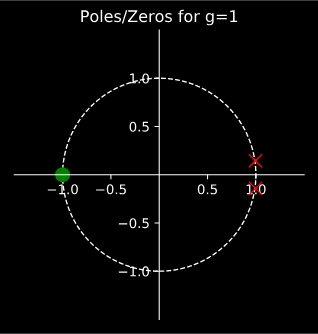
\includegraphics[width=1.7in]{../Pics/pz1.png}
    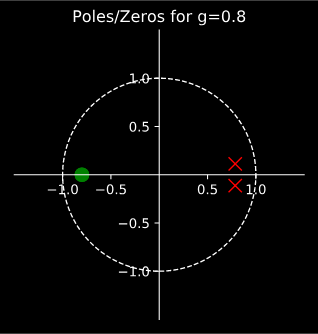
\includegraphics[width=1.7in]{../Pics/pz08.png}
    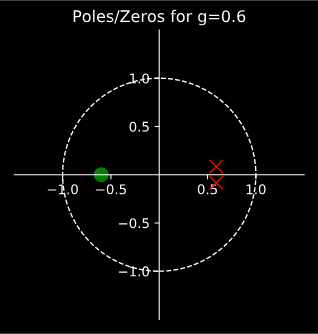
\includegraphics[width=1.7in]{../Pics/pz06.png}
    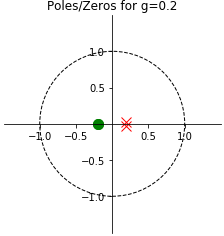
\includegraphics[width=1.7in]{../Pics/pz02.png}
    \caption{\label{pzPlots}{\it Instantaneous poles for a nonlinear biquad resonant
                                lowpass filter calculated from \cref{eq:poles_nl}, with
                                $g_1 = g_2 = g$.}}
\end{figure*}
%
We now propose a different structure for adding elements to a TDF-II
Biquad filter, this time adding nonlinear elements to the feedback
paths (see \cref{NL2-TDF-II}). Note that though the two structures are developed
separately here, they could certainly be combined into a third structure,
which will also be stable under the same conditions as the two original
structures.
%
\begin{figure}[ht]
    \center
    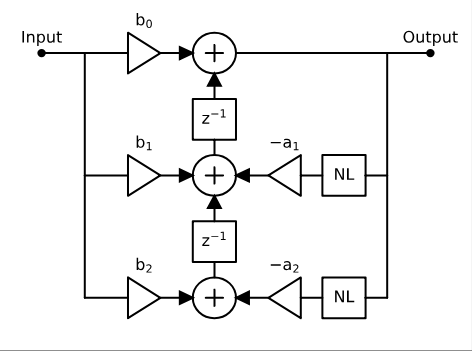
\includegraphics[width=2.3in]{../../NonlinearFeedback/Pics/NL2-TDF-II-White.png}
    \caption{\label{NL2-TDF-II}{\it Nonlinear Feedback Filter.}}
\end{figure}
%
The equaton for the filter can now be written:
%
\begin{equation}
    \begin{split}
        y[n] &= b_0 u[n] + b_1 u[n-1] + b_2 u[n-2] \\
             &- a_1 f_{NL}(y[n-1]) - a_2 f_{NL}(y[n-2])
    \end{split}
        \label{eq:nlbq2}
\end{equation}
%
Again, we can replace the nonlinear elements with their linearized
models, this time using the $y[n-1]$ and $y[n-2]$ terms to define our
operating points.
%
\begin{equation}
    \begin{split}
        & \bar{f}_{NL_k}(x) = g_k x + \gamma_k \\
        & g_k = f'_{NL}(y[n-k]), \; \gamma_k = c(y[n-k])
    \end{split}
        \label{eq:gs2}
\end{equation}
%
And again, the filter equation can be re-written:
%
\begin{equation}
    \begin{split}
        y[n] & = b_0 u[n] + b_1 u[n-1] + b_2 u[n-2] \\
        & - a_1 (g_1 y[n-1] + \gamma_1)
        - a_2 (g_2 y[n-2] + \gamma_2)
    \end{split}
        \label{eq:nlbq2_rewrite}
\end{equation}
%
Or by re-writing the filter coefficients, we see:
%
\begin{align}
    \begin{split}
        b_0' &= b_0\\
        b_1' &= b_1\\
        b_2' &= b_2\\
        a_1' &= g_1 a_1\\
        a_2' &= g_2 a_2
    \end{split}
        \label{eq:bq2_coefs_re-write}
\end{align}
%
\begin{equation}
    \begin{split}
        y'[n] &= b_0' u[n]
        + b_1' u[n-1] - a_1' y[n-1] \\
        & + b_2' u[n-2] - a_2' y[n-2]
        - a_1\gamma_1 - a_2\gamma_2
    \end{split}
        \label{eq:nlbq2_re-write2}
\end{equation}
%
Again, the $\gamma$ offset terms will not affect the filter stability.

\subsection{Stability}
%
We can now update \cref{eq:bq_lin_state_spaces} for the nonlinear
feedback filter described by \cref{eq:nlbq2}, and by writing it in the form
of \cref{eq:lyapunov_general}, we see
%
\begin{equation}
    \begin{bmatrix} x_1[n+1] \\ x_2[n+1] \\ y[n+1] \end{bmatrix} =
    \mathbf{h} \left( \begin{bmatrix} x_1[n] \\ x_2[n] \\ y[n] \end{bmatrix}
    \right) + \begin{bmatrix} b_1\\ b_2\\ b_0 \end{bmatrix} u[n]
    \label{eq:nlbq2_states}
\end{equation}
%
where
%
\begin{equation}
    \begin{split}
        h_1(x_1[n], x_2[n], y[n]) =& x_2[n] - a_1f_{NL}(y[n]) \\
        h_2(x_1[n], x_2[n], y[n]) =& -a_2f_{NL}(y[n]) \\
        h_3(x_1[n], x_2[n], y[n]) =& x_1[n]
    \end{split}
    \label{eq:nlbq2_state_eqns2}
\end{equation}
%
Then the Jacobian matrix can be written as:
%
\begin{equation}
    \mathbf{J} = \begin{bmatrix}
        0& 1& -a_1f'_{NL}(y[n]) \\
        0& 0& -a_2f'_{NL}(y[n]) \\
        1& 0& 0
    \end{bmatrix}
    \label{eq:nlbq2_Jacobian}
\end{equation}
%
Again, assuming that the corresponding linear filter is stable, the
nonlinear feedback filter will be stable provided the constraint
from \cref{eq:NL_constraint} is satisfied.
%
\begin{figure*}[!ht]
    % \center
    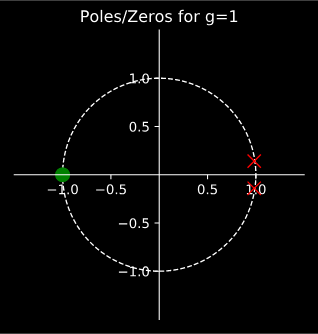
\includegraphics[width=1.7in]{../../NonlinearFeedback/Pics/pz1.png}
    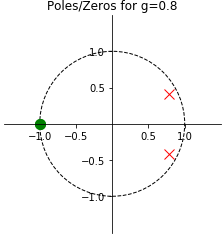
\includegraphics[width=1.7in]{../../NonlinearFeedback/Pics/pz08.png}
    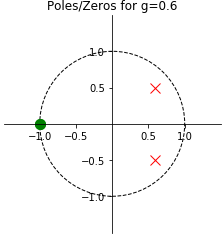
\includegraphics[width=1.7in]{../../NonlinearFeedback/Pics/pz06.png}
    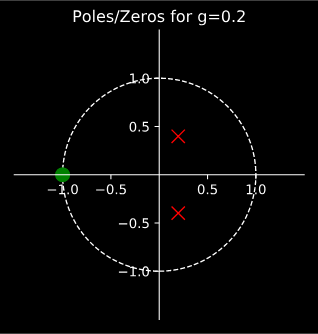
\includegraphics[width=1.7in]{../../NonlinearFeedback/Pics/pz02.png}
    \caption{\label{pzPlots2}{\it Instantaneous poles for a resonant
                                lowpass filter with nonlinear feedback,
                                calculated from \cref{eq:poles_nl2},
                                with $g_1 = g_2 = g$.}}
\end{figure*}
%

\subsection{Pole Analysis}
%
We can now calculate the locations of the instantaneous poles for
the nonlinear feedback filter, by adjusting the formula from
\cref{eq:poles_lin}.
%
\begin{equation}
p' = \frac{-g_1 a_1 \pm \sqrt{g_1^2 a_1^2 - 4 g_2 a_2}}{2}
    \label{eq:poles_nl2}
\end{equation}
%
In this case the pole magnitude and angle will move as follows:
\begin{equation}
    |p|^2 = g_2a_2
    \label{eq:poles_nl2_mag}
\end{equation}
%
\begin{equation}
    \angle p = \arctan \left( \pm \frac{\sqrt{4\frac{g_2}{g_1^2}a_2 - a_1^2}}{a_1} \right)
    \label{eq:poles_nl2_angle}
\end{equation}
%
Note that for saturating nonlinearities, the pole magnitude decays to
zero more slowly than for the
nonlinear biquad. More importantly, as the input gain increases,
the pole angle increases as well. \cite{Vadim} describes this sort of
pole movement as ``audio-rate modulation of the cutoff'' for the
filter, which can be a useful way of thinking about this phenomenon.
\newline\newline
Finally, note that unlike the nonlinear biquad, the zeros of the
filter are not affected by the nonlinear elements.
While adding nonlinear elements to the feedforward path can introduce 
a similar effect for the zeros, this would be
functionally equivalent to processing the signal through a nonlinearity
before passing it into the filter. Again, an example of this pole movement
can be seen in \cref{pzPlots2}.
%

\section{Example: Resonant Lowpass Filter}
%
As an example of the nonlinears structure developed above,
we will now examine a resonant lowpass filter
designed with both nonlinear structures. We will then show how the
nonlinear biquad structure can be useful for analog modelling,
and compare to an analog filter made with the same specifications.
\newline\newline
Our example filter will be a lowpass filter with a cutoff frequency
at $f_c = 1\text{ kHz}$, and $Q=10$. For our nonlinear elements, we
will use a hyperbolic tangent function $f_{NL}(x) = \tanh (x)$.
Note that this nonlinear function belongs to the class of
saturating nonlinearities described by \cref{eq:Sat_constraint}.
%
\begin{figure}[h]
    \center
    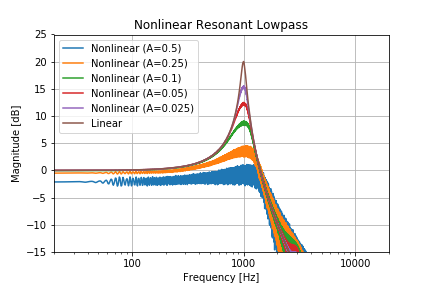
\includegraphics[width=3in]{../Pics/NL-LPF.png}
    \caption{\label{NL-LPF-freq}{\it Frequency responses of nonlinear biquad lowpass
                                    filters at varying amplitudes.}}
\end{figure}
%

\subsection{Digital Nonlinear Biquad}

We first construct this filter using the nonlinear biquad structure.
In \cref{NL-LPF-freq} we show the response of this filter for sine sweeps of
various amplitudes, compared to the frequency response of the corresponding
linear filter. In \cref{pzPlots} we show the movement of the poles and zeros of
the filter for varying steady state inputs. We calculate the instantaneous
poles using \cref{eq:poles_nl}, using $g_1 = g_2 = g$, as described in
each figure.
%
\begin{figure}[ht]
    \center
    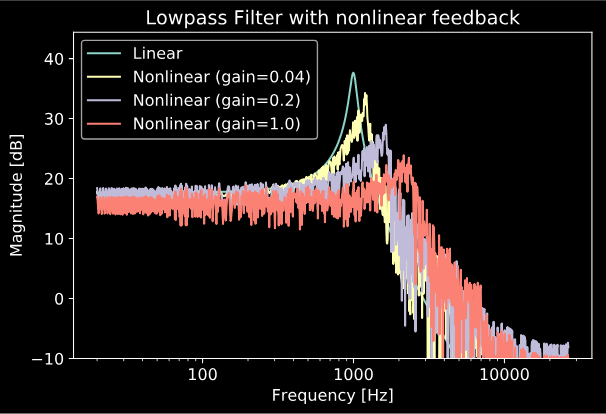
\includegraphics[width=3in]{../../NonlinearFeedback/Pics/LPF-NL.png}
    \caption{\label{NL2-LPF-freq}{\it Frequency responses of lowpass
                                    filters with nonlinear feedback
                                    at varying amplitudes.}}
\end{figure}
%

\subsection{Digital Nonlinear Feedback Filter}
%
Next, we construct the same resonant lowpass filter
using the nonlinear feedback structure. In \cref{NL2-LPF-freq},
we show the frequency response of the filter for sine sweeps of
various amplitudes. In \cref{pzPlots2} we show the movement of the
poles and zeros of the filter for various steady state gains. The
instantaneous poles are calculated using \cref{eq:poles_nl2}, again
using $g_1 = g_2 = g$.

\subsection{Using the Nonlinear Biquad for Analog Modelling}
%
To show how the nonlinear biquad filter structure can be useful
for analog modelling purposes, first note that the input gain to
the nonlinear biquad can be used as a tunable parameter (see \cref{50hz}).
\newline\newline
%
\begin{figure}[h]
    \center
    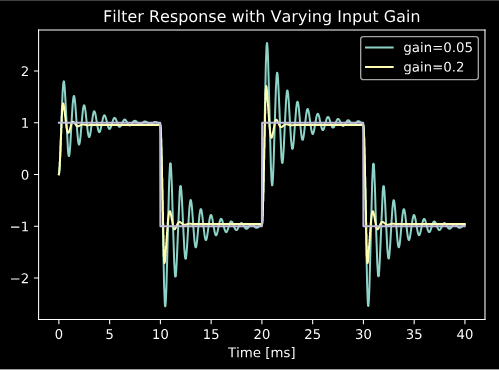
\includegraphics[width=3in]{../Pics/50-Hz_Response.png}
    \caption{\label{50hz}{\it Response of the nonlinear resonant lowpass
                            filter to a 50 Hz square wave with varying input gain.}}
\end{figure}
%
By tuning the input gain, we can attempt to match the response of an
arbitrary analog filter, either by tuning the parameters by ear
or using some form of numerical optimisation. Note that the choice
of base nonlinearities used by the nonlinear biquad will also play a
role in the accuracy of the model. For example, if the output of the
analog filter being modelled is asymmetric, then to accurately model
that filter, the nonlinear biquad must be constructed using
asymmetric base nonlinearities.
%

\subsubsection{Comparison with Analog Filter}

As an example, we can attempt to construct a naive model of a Sallen-Key
lowpass filter, a commonly used analog filter structure, and compare
our results to the desired analog response, similar to the
comparison done in \cite{SKF}. We describe this
as a naive model because we do not make any attempt to understand the physical
properties of the analog filter when constructing this model. We construct
a nonlinear biquad filter using $\tanh$ base nonlinearities, and design a
resonant lowpass filter with cutoff frequency $f_c = 1 \text{ kHz}$,
and $Q=10$, as well as a simulation of the corresponding Sallen-Key
filter using LTSpice. To accentuate the nonlinear behavior of the analog
filter, we choose $\pm 4 \text{ V}$ as the source voltages for the analog
filter circuit.
\newline\newline
We then compare the outputs of the two filters
for square waves at different frequencies, and use a simple staircase
optimisation scheme to find the input gain for the nonlinear biquad
that best matches the analog simulation. The results for the $250 \text{ Hz}$
square wave can be seen in \cref{SPICE}. While the nonlinear biquad model
is not perfect, it does capture the damping effects of the analog filter
much more accurately than the corresponding linear filter, and can be greatly
improved with a more well-informed choice of base nonlinear functions, and
a more sophisticated optimisation scheme.
%
\begin{figure}[ht]
    \center
    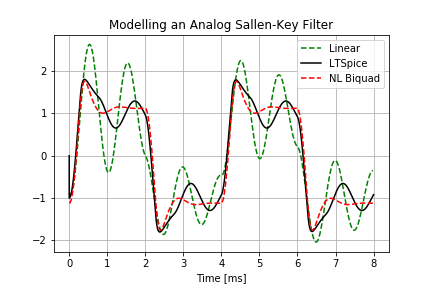
\includegraphics[width=3in]{../Pics/Spice-Compare.png}
    \caption{\label{SPICE}{\it Comparison between a linear resonant lowpass
                            filter, a resonant lowpass made with a nonlinear biquad
                            using a $\tanh$ clipper with input gain $0.283$,
                            and a SPICE simulation of a Sallen-Key lowpass.
                            All of the lowpass filters have $f_c=1$ kHz, and
                            $Q=10$. The input signal in each case is a $250$ Hz
                            square wave.}}
\end{figure}
%

\section{Conclusion}

In this paper, we have developed two structures for stable nonlinear biquad
filters. We have introduced the new architecture as a modification of the
Transposed Direct Form II filter structure, and shown
how the changed architecture affects the pole locations depending on
the amplitude of the input signal. We have also derived constraints under
which the structure is guaranteed stable.
\newline\newline
As a case study, we have implemented
a resonant lowpass filter using both nonlinear
structures, and shown that the
poles respond to the input as expected. We then show how the
nonlinear biquad structure can be used to model an analog
filter, comparing with a Sallen-Key lowpass filter as
an example. Note that while the nonlinear biquad structure
can be used for analog modelling, both structures can also be
used purely in the digital domain as a tool for constructing
filters that sound more sonically interesting and harmonically
rich.
\newline\newline
To demonstrate this last point, we have also developed an open-source
audio plugin (VST, AU) implentation of both the nonlinear biquad and
nonlinear feedback filters, extending to several filter shapes, and
several base nonlinearities.
The source code for the plugin implementation is available on
GitHub,\footnote{\url{https://github.com/jatinchowdhury18/ComplexNonlinearities}}
and video demonstrations are available on YouTube.\footnote{\url{https://youtu.be/BMzKdaZtmoU}}
\footnote{\url{https://youtu.be/T0AsIX5oL9A}}
\newline\newline
Future research concerning nonlinear filtering will center around making a
more informed choice of base nonlinearities, focusing on both the desired
harmonic response of the filter, as well as physically meaningful base
nonlinearities for use in analog modelling.

\section*{Acknowledgment}

The author would like to thank Kurt Werner for providing sound advice and
guidance on this topic, Viraga Perera and Dave Berners for informative
discussions, as well as the GASP working group at CCRMA.

\begin{thebibliography}{00}
\bibitem{JOSFilters} J. O. Smith, ``Introduction to Digital Filters with Audio Applications'' W3K Publishing, 2007.  Available: \underline {https://ccrma.stanford.edu/~jos/filters/}
\bibitem{SKF} R. Muller and T. Helie, ``A Minimal Passive Model of the Operational Amplifier: Application to  Sallen-Key Analog Filters,'' in \emph{Proc. of the 22nd Int. Conference on Digital Audio Effects}, 2019.
\bibitem{BLAMP} F. Esqueda, V. Valimaki, and S. Bilbao, ``Rounding Corners with BLAMP'', in \emph{Proc. of the 16th Int. Conference on Digital Audio Effects}, 2016.
\bibitem{Lyapunov} G. Chen, ``Stability of Nonlinear Systems'', 2005. Available: \underline{10.1002/0471654507.eme413}
\bibitem{Vadim} V. Zavalishin, ``The Art of VA Filter Design'' 2018, pp. 173--236.% Available: \underline{https://native-instruments.com/fileadmin/ni\_media/downloads/pdf/VAFilterDesign\_2.0.0a.pdf}
\bibitem{Rossum1992MakingDF} D. Rossum, ``Making Digital Filters Sound "Analog",'' in \emph{Int. Computer Music Conference}, 1992.
\bibitem{BernersDAFX} D. Berners, ``Modeling Circuits with Nonlinearities in Discrete Time,'' presented at the \emph{20th Int. Conference on Digital Audio Effects}, 2017. Available: \underline{https://www.youtube.com/watch?v=7Npx0eaSxow}
\bibitem{LyapunovFixedPointFilters} K. Erickson and A. Michel, ``Stability analysis of fixed- point digital filters using computer generated Lyapunov functions- Part I: Direct form and coupled form filters,'' \emph{IEEE Trans. on Circuits and Systems}, Vol. 32, pp. 113-132, 1985.
\bibitem{JOS-Waveguide} J. O. Smith and D. Rocchesso, ``Aspects of Digital Waveguide Networks for Acoustic Modeling Applications'', 2010. Available: \underline{https://ccrma.stanford.edu/~jos/wgj/wgj.html}
\end{thebibliography}

\begin{IEEEbiographynophoto}{Jatin Chowdhury} received a B.S. degree in
electrical engineering from the University of Southern California, in Los
Angeles, California, USA, in 2018,
majoring in circuits, signals, and systems, and minoring in physics, and
music recording. Mr. Chowdhury is currently completing a M.A. in
music, science, and technology at Stanford University, in Stanford,
California, USA.

He has previously worked as an electrical engineer, STEM educator,
audio software engineer, and astrophysics researcher. His current
research typically deals with nonlinear signal processing systems,
often with the end goal of creating real-time systems for processing
or sythesizing digital audio. His broader research interests include
adaptive signal processing, embedded signal processing, and physical
modelling signal processing.
\end{IEEEbiographynophoto}

\end{document}
